\documentclass{article}

% Paquetes que se usan en el template
\usepackage[utf8]{inputenc} % Required for inputting international characters
\usepackage[T1]{fontenc} % Output font encoding for international characters
\usepackage{mathpazo} % Palatino font
\usepackage{listings}
\usepackage{graphicx}
\usepackage{fancybox}
\usepackage[a4paper]{geometry}

\geometry{top=2cm, bottom=2cm, left=2.5cm, right=2.5cm}
\renewcommand{\figurename}{Captura}

\begin{document}

%----------------------------------------------------------------------------------------
%	TITLE PAGE
%----------------------------------------------------------------------------------------

\begin{titlepage} % Suppresses displaying the page number on the title page and the subsequent page counts as page 1
	\newcommand{\HRule}{\rule{\linewidth}{0.4mm}} % Defines a new command for horizontal lines, change thickness here
	
	\center % Centre everything on the page
	
	%------------------------------------------------
	%	Headings
	%------------------------------------------------
	
	\textsc{\Huge Algoritmos y Programaci\'on I}\\[2.5cm] % Main heading such as the name of your university/college
	
	\textsc{\Large C\'atedra Diego Essaya}\\[0.8cm]  % Major heading such as course name 
	
	\textsc{\large Pr\'actica Alan}\\[3.5cm] % Minor heading such as course title
	
	%------------------------------------------------
	%	Title
	%------------------------------------------------
	
	\HRule\\[0.4cm]
	
	{\huge\bfseries Trabajo Pr\'actico III}\\[0.4cm] % Title of your document
	
	\HRule\\[3.5cm]
	
	%------------------------------------------------
	%	Author(s)
	%------------------------------------------------

	\begin{minipage}{0.4\textwidth}
		\begin{flushleft}
			\Large
			\textit{Alumnos:}\\[0.4cm] % Mi nombre y legajo
			\textit{Guerra, Lucas}\\
			\textit{Legajo: 104096}\\[0.2cm]
			
			\textit{Patrone, Florencia}\\
			\textit{Legajo: 102863}\\
		\end{flushleft}
	\end{minipage}
	~
	\begin{minipage}{0.4\textwidth}
		\begin{flushright}
			\Large
			\center \textit{Corrector}\\
			Mart\'in Margonari % Nombre del ayudante
		\end{flushright}
	\end{minipage}
	
	
	
	%------------------------------------------------
	%	Fecha
	%------------------------------------------------
	
	\vfill\vfill\vfill % Position the date 3/4 down the remaining page
	{\large Fecha de entrega :} 
	{\large  03 de Junio del 2019} % Date, change the \today to a set date if you want to be precise
	
	%------------------------------------------------
	%	Logo
	%------------------------------------------------
	
	%\vfill\vfill
	%\includegraphics[width=0.2\textwidth]{placeholder.jpg}\\[1cm] % Include a department/university logo - this will require the graphicx package
	 
	%----------------------------------------------------------------------------------------
	
	\vfill % Push the date up 1/4 of the remaining page
	
\end{titlepage}

%----------------------------------------------------------------------------------------
% Parte 1 - Enunciado del TP3
%----------------------------------------------------------------------------------------

\begin{Huge}
	\begin{center}
		\textbf{Fractales \\[1cm]}
	\end{center}	 
\end{Huge}




\begin{description}
	\item \textbf{Consigna} \\ Implementar un programa que permita generar im\'agenes fractales, mediante un algoritmo basado en sistemas-L, una simulaci\'on de gr\'aficos tortuga y el formato de im\'agenes est\'andar SVG. \\[0.5cm]
	\begin{center}
		\textbf{Referencias \\[1cm]}
	\end{center}	 
	 \item \textbf{Relas} \\ El juego se desarrolla en un tablero compuesto por una grilla rectangular de celdas. Cada celda puede contener o no una mina. Todas las celdas est\'an inicialmente cubiertas, y el objetivo consiste en descubrir todas las que no est\'en ocupadas por minas.\\
\end{description}

	\begin{itemize}
		\item El juego comienza con todas las celdas cubiertas. Cada celda puede estar ocultando tanto una mina como un espacio vac\'io\\
		\item El jugador puede descubrir una celda por vez.\\
			\begin{itemize}
				\item Si se descubre un espacio que contiene una mina el juego finaliza. \\
				\item Si se selecciona un lugar vac\'io debe mostrarse la cantidad de minas que tiene a su alrededor esa posici\'on. (Nota: A diferencia del Buscaminas original, los casilleros que no tengan minas a su alrededor no reaccionar\'an en cadena con sus adyacentes)
			\end{itemize}
		\item En cualquier momento el jugador puede colocar o quitar banderas en celdas cubiertas. Una celda marcada con una bandera sirve para indicar que probablemente contiene una mina. \\	
			\begin{itemize}
				\item Una celda marcada con una bandera no puede ser descubierta.
			\end{itemize}
		\item El juego termina cuando todas las celdas que no contienen minas hayan sido descubiertas.
	
	\end{itemize}
 \newpage
 
 
 \begin{Huge}
	\begin{center}
		\textbf{Concluciones \\[1cm]}
	\end{center}	 
\end{Huge}

\begin{description}
	\item \textbf{Desaf\'ios}\\
		
		\begin{itemize}
			\item Uno de los primeros inconvenientes con los que me top\'e fue como imprimir los \'indices del tablero, hace mucho no lo hac\'ia, y me robo un poco de tiempo acomodarlos dentro de los b\'ucles con los que recorr\'ia el tablero.
			\item Para poder operar sobre el tablero y a la vez ir mostr\'andoselo al usuario, resolv\'i utilizar dos, para separar la l\'ogica y tambi\'en para poder hacer pruebas, visualizando en que lugar estaban las minas.
			\item A la hora de colocar las minas en el tablero, utilic\'e la librer\'a \textbf{random} para darle un poco de azar a la selecci\'on de los \'indices. Adem\'as de devolverme el tablero con las minas cargadas, mi funci\'on me devuelve una tupla con las ubicaciones de las minas, esto agiliza en parte las consultas. Use tuplas para no mandarme alguna macana y cambiarles el valor por error.
			\item Quiz\'as el desaf\'io mas interesante fue el de validar lo que el usuario ingresaba, utilizando la funcion \Ovalbox{\bf  search} de la libreria de expresiones regulares de Python, logr\'e verificar si lo que el usuario ingreso coincidia con el patr\'on \textbf{fila - columna - bandera} . La funci\'on \Ovalbox{\bf  search} devuelve los valores ingresados, separados en una especie de grupo, lo que permite accederlos a traves de un \'indice. Bastante limpia y pr\'actica.
			\item Punto que no termine de entender, y tampoco encontr\'e mucha informaci\'on fue acerca del funcionamiento de las banderas, si bien mi buscaminas permite colocarlas y retirarlas (informando cuando se lo hace), no les d\'i otra utilidad.
			\item Por \'ultimo, en lo que m\'as tiempo \''invert\'i\'', fu\'e en la b\'usqueda de las minas adyacentes, intent\'e no utilizar demasiadas l\'ineas de c\'odigo, pero el objetivo principal era que el programa funcione y no se rompa por un \'indice fuera de rango.
		\end{itemize}

\end{description}

\newpage

\begin{figure}[hbt!]
	\center
	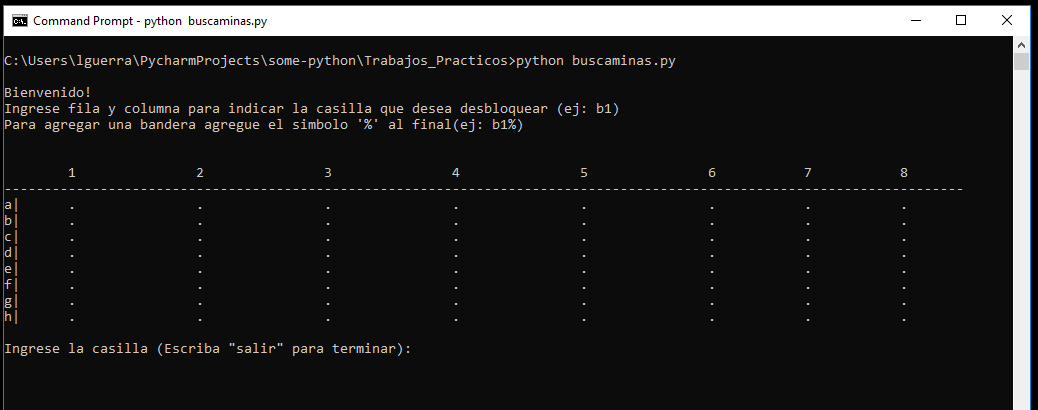
\includegraphics[width=1\textwidth]{img/ejecucion_cmd.PNG}
	\caption{
	\label{fig:my-label} Ejecuci\'on en consola. }
\end{figure}

\begin{figure}[hbt!]
	\center
	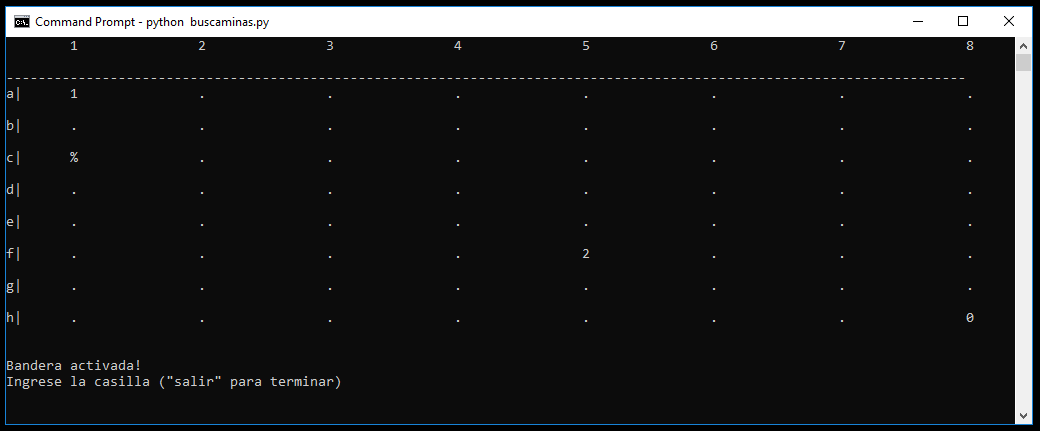
\includegraphics[width=1\textwidth]{img/ejecucion_cmd2.PNG}
	\caption{
	\label{fig:my-label} Ejecuci\'on en consola. }
\end{figure}


\begin{flushright}
	Informe escrito con \Ovalbox{\bf \LaTeX}
\end{flushright}

\end{document}
\grid